\documentclass[12pt]{article}

\usepackage{sbc-template}
% \usepackage{graphicx,url}
\usepackage[utf8]{inputenc}
%\usepackage[brazil]{babel}
\usepackage{graphicx}
\usepackage{float}
\usepackage{subfig}
\usepackage{amsmath}

\sloppy

\title {
	Métodos de Particionamento de Grafos Aplicados à Segmentação de Imagens
}

\author {
	Lucas Gualtieri \inst{1},
	Gabriel Felipe Quaresma de Oliveira \inst{1}, \\
	Pedro Rodrigues Alves \inst{1},
	Vitor Lúcio de Oliveira \inst{1},
}

\address {
	Pontifical Catholic University of Minas Gerais\\
	Coração Eucarístico -- 30535-901 -- Belo Horizonte -- MG -- Brazil
	\email{\{gabrielqoliveira, vitor.lucio.0916\}@gmail.com,}
	\email{\{lgualtieri, pedro.alves.1446100\}@sga.pucminas.br}
}

\begin{document} 

\maketitle

\begin{resumo} 
	Este meta-artigo descreve o estilo a ser usado na confecção de artigos e
	resumos de artigos para publicação nos anais das conferências organizadas
	pela SBC. É solicitada a escrita de resumo e abstract apenas para os artigos
	escritos em português. Artigos em inglês deverão apresentar apenas abstract.
	Nos dois casos, o autor deve tomar cuidado para que o resumo (e o abstract)
	não ultrapassem 10 linhas cada, sendo que ambos devem estar na primeira
	página do artigo.
\end{resumo}

\section{Introdução}
A segmentação de imagens é um dos desafios mais significativos na área de visão computacional, desempenhando um papel crucial na análise e interpretação de dados visuais. A capacidade de dividir uma imagem em regiões significativas permite que algoritmos de visão computacional realizem tarefas complexas, como reconhecimento de objetos, rastreamento e compreensão de cenas. Nos últimos anos, abordagens baseadas em grafos têm emergido como uma solução promissora para o problema de segmentação, oferecendo uma estrutura matemática robusta para modelar as relações entre pixels e suas características. Este artigo explora as técnicas de segmentação de imagens utilizando algoritmos baseados em grafos, destacando suas vantagens em capturar aspectos globais da imagem e sua eficiência computacional.

A segmentação de imagens não é apenas uma questão de dividir uma imagem em partes, mas também envolve a definição de critérios que determinam a qualidade e a precisão da segmentação. A introdução de algoritmos que utilizam cortes de grafos, como o método de cortes normalizados, tem contribuído significativamente para o avanço nesta área, permitindo segmentações que preservam detalhes em regiões de baixa variabilidade enquanto ignoram detalhes em regiões de alta variabilidade. Este trabalho se baseia em tais abordagens, apresentando um algoritmo eficiente que se adapta a diferentes tipos de imagens e condições.

\section{Trabalhos Relacionados}
A literatura sobre segmentação e agrupamento é vasta,
com contribuições significativas ao longo das últimas três décadas.
Cooper discute a tratabilidade da segmentação e análise de cenas,
abordando as complexidades envolvidas na definição de critérios de segmentação eficazes.
O trabalho de \cite{felzenszwalb2004efficient} apresenta um algoritmo de segmentação baseado
em grafos que mede a evidência de limites entre regiões, utilizando uma representação gráfica da imagem.
Este algoritmo é notável por sua eficiência, operando em tempo quase linear em relação ao número de
arestas do grafo, e por sua capacidade de produzir segmentações que satisfazem propriedades globais,
mesmo ao tomar decisões gulosas.

Além disso, a abordagem de Felzenszwalb e Huttenlocher é contextualizada dentro de um amplo espectro
de métodos de segmentação, incluindo técnicas de fusão de regiões e métodos baseados em cortes de grafos,
que têm sido amplamente explorados na literatura. Esses métodos representam a segmentação como um problema
de otimização em um grafo, onde cada pixel é um nó e as arestas representam a relação entre pixels vizinhos.
A combinação dessas abordagens tem levado a avanços significativos na segmentação de imagens, permitindo
uma melhor compreensão e análise de cenas complexas.

Boykov e Funka-Lea propuseram um framework de segmentação utilizando cortes de grafo (\textit{s/t graph cuts}), destacando sua eficiência para otimização global, robustez numérica e capacidade de integrar pistas baseadas em bordas e regiões \cite{boykov2006graph}. Esse trabalho estabeleceu conexões com métodos anteriores, como contornos ativos e conjuntos de nível, mostrando que a abordagem de cortes de grafo pode ser vista como uma contraparte discreta desses métodos.

Além disso, os autores demonstraram a aplicabilidade do framework para imagens N-dimensionais e sua flexibilidade em integrar informações de contexto, propriedades regionais e restrições topológicas. O método foi aplicado com sucesso em problemas como segmentação de objetos em imagens naturais e dados médicos, evidenciando sua utilidade em uma ampla gama de aplicações \cite{boykov2006graph}.

O trabalho de Boykov e Funka-Lea destaca como o particionamento de grafos é uma ferramenta poderosa e versátil para segmentação de imagens, proporcionando uma base sólida para o desenvolvimento de algoritmos eficientes e robustos.

\section{Metodologia}
Para implementar os algoritmos descritos nos artigos \cite{boykov2006graph} e \cite{felzenszwalb2004efficient}, a imagem no formato PPM foi convertida em uma matriz de pixels no espaço RGB. Em seguida, diferentes estruturas de dados foram empregadas para cada um dos algoritmos, conforme suas especificidades. 

\subsection{Primeiro Artigo}

A implementação dos autores \cite{felzenszwalb2004efficient} mantém a segmentação \( S \) utilizando uma floresta de conjuntos disjuntos com união por rank e compressão de caminho. O tempo de execução do algoritmo pode ser dividido em duas partes. Primeiramente, no Passo 0, é necessário ordenar os pesos em ordem não decrescente. Para pesos inteiros, isso pode ser feito em tempo linear utilizando ordenação por contagem (\textit{counting sort}), e, em geral, pode ser feito em \( O(m \log m) \) usando qualquer um dos diversos métodos de ordenação.

Os Passos 1-3 do algoritmo requerem \( O(m \alpha(m)) \) de tempo, onde \( \alpha \) é a função inversa de Ackermann, que cresce de forma extremamente lenta. Para verificar se dois vértices estão no mesmo componente, usamos a operação \textit{set-find} em cada vértice, e para unir dois componentes, utilizamos a operação \textit{set-union}. Assim, há no máximo três operações de conjuntos disjuntos por aresta. O cálculo de \( MInt \) pode ser feito em tempo constante por aresta se conhecermos \( Int \) e o tamanho de cada componente.

\subsubsection{Estruturas de Dados Utilizadas}

Para a segmentação de imagens, utilizamos um grafo não direcionado \( G = (V, E) \), onde os nós \( V \) representam os pixels da imagem e as arestas \( E \) conectam pares de pixels vizinhos. Cada aresta \( (v_i, v_j) \in E \) possui um peso \( w((v_i, v_j)) \), que é uma medida da dissimilaridade entre os pixels conectados por essa aresta. No caso de segmentação de imagens, o peso da aresta pode ser baseado na diferença de intensidade, cor, movimento, localização ou algum outro atributo local dos pixels.

\subsubsection{Algoritmo de Segmentação}

O algoritmo de segmentação proposto baseia-se na comparação de regiões pares para determinar a evidência de uma fronteira entre duas componentes. A diferença entre duas componentes \( C_1 \) e \( C_2 \) é definida como o peso mínimo da aresta que conecta essas duas componentes:

\[
\text{Dif}(C_1, C_2) = \min_{v_i \in C_1, v_j \in C_2, (v_i, v_j) \in E} w((v_i, v_j))
\]

A diferença interna de uma componente \( C \) é definida como o maior peso na árvore geradora mínima (MST) da componente:

\[
\text{Int}(C) = \max_{e \in \text{MST}(C, E)} w(e)
\]

O algoritmo utiliza um predicado de comparação de regiões para avaliar se há evidência de uma fronteira entre duas componentes, comparando a diferença entre as componentes com a diferença interna de pelo menos uma das componentes. Um limiar é usado para controlar o grau de diferença necessário para que haja evidência de uma fronteira:

\[
D(C_1, C_2) = \begin{cases} 
\text{true} & \text{se } \text{Dif}(C_1, C_2) > \text{MInt}(C_1, C_2) \\
\text{false} & \text{caso contrário}
\end{cases}
\]

onde a diferença interna mínima \( \text{MInt} \) é definida como:

\[
\text{MInt}(C_1, C_2) = \min(\text{Int}(C_1) + \tau(C_1), \text{Int}(C_2) + \tau(C_2))
\]

A função de limiar \( \tau \) é baseada no tamanho da componente:

\[
\tau(C) = \frac{k}{|C|}
\]

onde \( |C| \) é o número de elementos em \( C \) e \( k \) é um parâmetro constante.

\subsubsection{Passos do Algoritmo}

\begin{enumerate}
    \item \textbf{Construção do Grafo}: Criamos um grafo onde cada pixel é um nó e adicionamos arestas entre pixels vizinhos com pesos baseados na dissimilaridade.
    \item \textbf{Ordenação das Arestas}: Ordenamos as arestas em ordem crescente de peso.
    \item \textbf{Inicialização}: Começamos com uma segmentação onde cada pixel é uma componente separada.
    \item \textbf{Iteração}: Para cada aresta na ordem ordenada, verificamos se as componentes conectadas pela aresta devem ser unidas com base no predicado de comparação de regiões. Se a condição for satisfeita, unimos as componentes.
    \item \textbf{Resultado}: A segmentação final é obtida após processar todas as arestas.
\end{enumerate}

\subsubsection{Vantagens do Método}

\begin{itemize}
    \item \textbf{Eficiência}: O algoritmo é altamente eficiente, com complexidade de tempo \( O(m \log m) \), onde \( m \) é o número de arestas no grafo.
    \item \textbf{Preservação de Detalhes}: O método preserva detalhes em regiões de baixa variabilidade enquanto ignora detalhes em regiões de alta variabilidade.
    \item \textbf{Adaptabilidade}: A abordagem adaptativa permite que o algoritmo capture características globais importantes da imagem, mesmo fazendo decisões gananciosas.
\end{itemize}

\subsection{Segundo Artigo}
Para a segmentação de imagens N-D, utilizamos um grafo \( G = (V, E) \) onde os nós \( V \) representam os pixels (ou voxels) da imagem e as arestas \( E \) conectam os nós vizinhos. Existem dois tipos principais de arestas:

\begin{itemize}
    \item \textbf{n-links (arestas de vizinhança)}: Conectam pares de pixels vizinhos e são usadas para representar a continuidade espacial na imagem.
    \item \textbf{t-links (arestas de terminal)}: Conectam cada pixel a dois nós terminais especiais, a fonte \( S \) (representando o objeto) e o sumidouro \( T \) (representando o fundo).
\end{itemize}

Cada aresta \( e \in E \) é associada a um peso \( w_e \), que reflete a penalidade de cortar essa aresta. Os pesos das n-links são baseados nas diferenças de intensidade entre pixels vizinhos, enquanto os pesos das t-links são determinados pelas propriedades regionais dos pixels.

\subsubsection{Algoritmo de Segmentação}

O algoritmo de segmentação proposto baseia-se na minimização de uma função de energia que combina propriedades de borda e região. A função de energia \( E(A) \) é definida como:

\[
E(A) = \lambda \sum_{p \in P} R_p(A_p) + \sum_{\{p,q\} \in N} B_{p,q} \cdot \delta(A_p \neq A_q)
\]

onde:
\begin{itemize}
    \item \( R_p(A_p) \) é o termo regional que penaliza a atribuição de um pixel \( p \) ao objeto ou ao fundo com base em modelos de intensidade.
    \item \( B_{p,q} \) é o termo de borda que penaliza a descontinuidade entre pixels vizinhos \( p \) e \( q \).
    \item \( \lambda \) é um coeficiente que controla a importância relativa dos termos regionais e de borda.
\end{itemize}

Para encontrar a segmentação ótima, utilizamos o algoritmo de corte de grafo s-t (source-to-sink), que é eficiente e garante a obtenção de uma solução globalmente ótima. O processo envolve os seguintes passos:

\begin{enumerate}
    \item \textbf{Construção do Grafo}: Criamos um grafo onde cada pixel é um nó e adicionamos arestas de vizinhança (n-links) e terminais (t-links) com pesos apropriados.
    \item \textbf{Cálculo do Corte Mínimo}: Aplicamos o algoritmo de fluxo máximo/corte mínimo para encontrar o corte que minimiza a função de energia. Este corte separa os nós terminais \( S \) e \( T \), resultando na segmentação da imagem em objeto e fundo.
    \item \textbf{Ajuste de Restrições}: Podemos adicionar restrições duras (seeds) para melhorar a segmentação, especificando pixels que devem pertencer ao objeto ou ao fundo. Estas restrições são incorporadas ajustando os pesos das t-links correspondentes.
\end{enumerate}

\subsubsection{Vantagens do Método}

\begin{itemize}
    \item \textbf{Ótima Global}: O uso de cortes de grafo garante que a segmentação encontrada seja globalmente ótima em relação à função de energia definida.
    \item \textbf{Flexibilidade}: O método pode ser aplicado a imagens de qualquer dimensão (2D, 3D, etc.) e permite a incorporação de várias pistas visuais e informações contextuais.
    \item \textbf{Eficiência}: Algoritmos de fluxo máximo/corte mínimo são eficientes e podem ser acelerados para aplicações dinâmicas e em tempo real.
\end{itemize}


\subsection{Geração de imagem saida}
Após a segmentação ser realizada, calcula-se a média das cores de cada componente na imagem original.A média das cores de cada componente \( C_j \) é dada por:

\[
\bar{r}_j = \frac{1}{|C_j|} \sum_{(i, j) \in C_j} r_i, \quad \bar{g}_j = \frac{1}{|C_j|} \sum_{(i, j) \in C_j} g_i, \quad \bar{b}_j = \frac{1}{|C_j|} \sum_{(i, j) \in C_j} b_i
\]

Onde:
- \( |C_j| \) é o número de pixels no componente \( C_j \),
- \( r_i, g_i, b_i \) são as componentes RGB do pixel \( i \) pertencente ao componente \( C_j \).

A cor média de cada região \( C_j \) é então usada para preencher toda a região com a cor:

\[
\text{Cor}(C_j) = (\bar{r}_j, \bar{g}_j, \bar{b}_j)
\]



\section{Resultados}

\begin{figure}[H]
    \centering
    \subfloat[Original]{
\includegraphics[width=0.45\linewidth]{images/input/paper.png}\label{fig:antes}} \hfill
    \subfloat[Segmentada]{
\includegraphics[width=0.45\linewidth]{images/output/paper.png}\label{fig:depois}}
    
    
\end{figure}
 Uma imagem sintética com três regiões perceptualmente distintas, e as três maiores regiões encontradas pelo nosso método de segmentação (parâmetros do algoritmo $\sigma = 0.8, k = 100.000$, ).

 \begin{figure}[H]
    \centering
    \subfloat[Original]{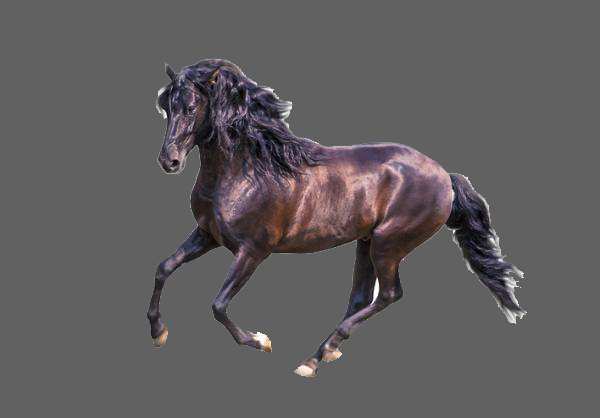
\includegraphics[width=0.45\linewidth]{images/input/cavalo.png}\label{fig:antes}} \hfill
    \subfloat[Segmentada]{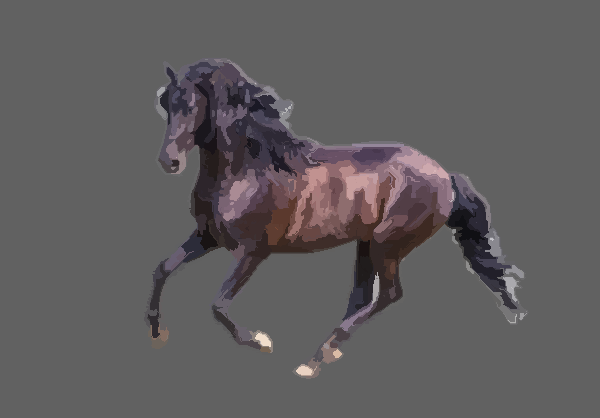
\includegraphics[width=0.45\linewidth]{images/output/cavalo.png}\label{fig:depois}}
    
    
\end{figure}
 Uma cena de um cavalo, as regiões encontradas pelo nosso método de segmentação (parâmetros do algoritmo $\sigma = 0.8, k = 300$, ).

 \begin{figure}[H]
    \centering
    \subfloat[Original]{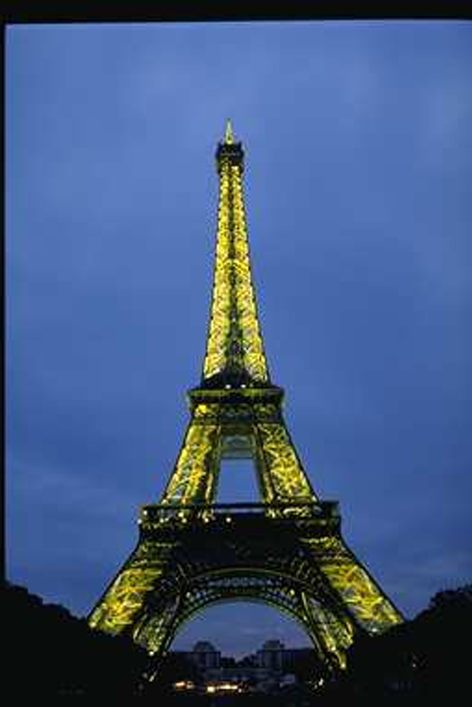
\includegraphics[width=0.45\linewidth]{images/input/torre.png}\label{fig:antes}} \hfill
    \subfloat[Segmentada]{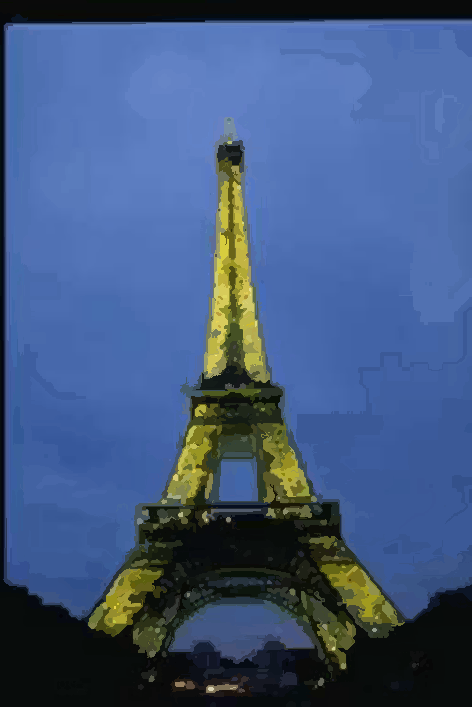
\includegraphics[width=0.45\linewidth]{images/output/torre.png}\label{fig:depois}}
    
    
\end{figure}
 Uma foto da Torre Eiffel, e as regiões encontradas pelo nosso método de segmentação (parâmetros do algoritmo $\sigma = 0.8, k = 300$, ).

 \begin{figure}[H]
    \centering
    \subfloat[Original]{\includegraphics[width=0.45\linewidth]{images/input/crosswalk.png}\label{fig:antes}} \hfill
    \subfloat[Segmentada]{\includegraphics[width=0.45\linewidth]{images/output/crosswalk.png}\label{fig:depois}}
    
    
\end{figure}
 Uma foto de um cruzamento, e as regiões encontradas pelo nosso método de segmentação (parâmetros do algoritmo $\sigma = 0.8, k = 600.000$, ).
 
 
\section{Conclusão}
Neste trabalho, exploramos métodos de particionamento de grafos aplicados à segmentação de imagens, baseando-nos nos algoritmos propostos por Felzenszwalb e Huttenlocher \cite{felzenszwalb2004efficient} e Boykov e Funka-Lea \cite{boykov2006graph}. Através da implementação e análise desses métodos, demonstramos a eficácia e a eficiência dos algoritmos de segmentação baseados em grafos em capturar características globais e preservar detalhes importantes das imagens.

O algoritmo de Felzenszwalb e Huttenlocher mostrou-se altamente eficiente, operando em tempo quase linear em relação ao número de arestas do grafo. Sua capacidade de ajustar adaptativamente o critério de segmentação com base na variabilidade das regiões vizinhas permitiu a obtenção de segmentações que satisfazem propriedades globais, mesmo ao tomar decisões gulosas. Além disso, é um método simples de se aplicar, pois não necessita de pré-processamento. Este método é particularmente eficaz em lidar com variações de intensidade e preservar detalhes em regiões de baixa variabilidade. 

Por outro lado, o framework de Boykov e Funka-Lea, apesar de ser uma idéia interessante e usar \textit{min-cut} e \textit{max-flow} para segmentar imagens, destacou-se pela sua dificuldade de implementação e dependência de informações adicionais das probabilidades de um vértice ser \textit{background} ou \textit{foreground}. Portanto, os resultados alcançados não foram os desejados.

Para concluir, os experimentos realizados evidenciam as vantagens e limitações de cada abordagem de particionamento de grafos no contexto da segmentação de imagens. Esses resultados sugerem que, enquanto os métodos baseados em \textit{min-cut} e \textit{max-flow} podem ser eficazes em cenários específicos, abordagens mais simples, como a de Felzenszwalb e Huttenlocher, continuam a ser preferidas para aplicações gerais de segmentação de imagens, especialmente quando a eficiência computacional é uma preocupação.


\bibliographystyle{sbc}
\bibliography{sbc-template}

\end{document}